\chapter{Experimental Mode Matching Cavities at Syracuse}
In conjunction with Sandoval et al \cite{Fabian_Thesis}, the table-top adaptive mode matching experiment was able to show the feasibility of a fully dynamical system at Syracuse University.  Most of the work done by the author was focused on converting and upgrading the real-time digital sysem (RTCDS) from being used by the optical trap experiment \cite{OpticalTrap} to adaptive mode matching and interfacing the RF sensors into the digital system.  There is also a section on the usage of cylindrical lenses and quadrant photodiodes as a viable method of extracting a mode matching error signal.

\section{Commissioning the Real Time Digital System}
	Dynamic control systems require both actuators and sensors which are interfaced in a real-time manner and this requires the use of analog-to-digital (ADC) and digital-to-analog (DAC) converters.  A LIGO standard system uses a front end computer that reads in data and processes the signals based off a Simulink graphical model that allows for simple logic, mathematical operations, and frequency dependent filtering.  The real time data acquisition code is user-interfaced with a Motif Editor and Display Manager (MEDM) that is able to report and execute variables such as gains and matrix elements.
	
	\begin{figure}[h]
		\centering
		\frame{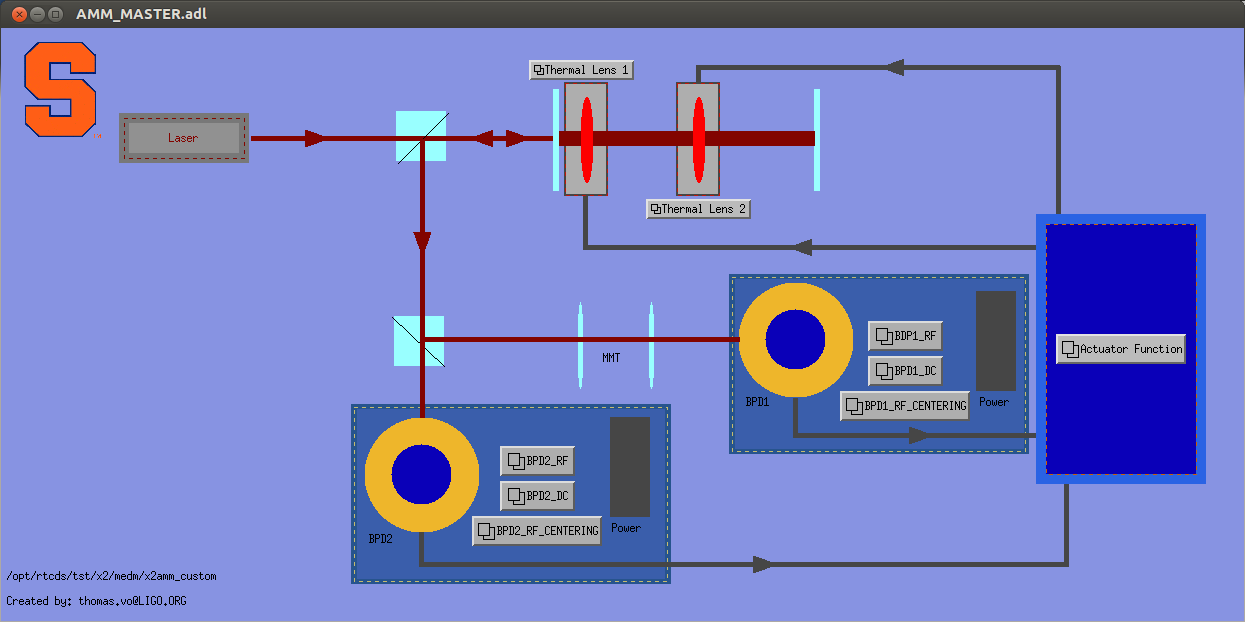
\includegraphics[width=1.0 \textwidth]{../Figures/AMM_MASTER.png}}
		\caption[MEDM master screen for adaptive mode matching at Syracuse.]
		{\textbf{MEDM master screen for adaptive mode matching at Syracuse.}  
			Here, the demodulated error signal in reflection of the Fabry-Perot cavity is divided by a beamsplitter and fed into two RF detectors, one of which is depicted to have a mode matching telescope MMT to project a different Gouy phase to sense an orthogonal degree of freedom. Then the signal is sent to an actuator function which allows for diagonalizing the signals and can be sent to a set of thermal lens at different Gouy phases for actuation.  The adaptive lenses are actually placed in the beam path before entering the cavity but for demonstrative purposes, they are portrayed at two different Gouy phases of the resonator.
		}
		\label{fig:AMM_Master}
	\end{figure}

	\section{Sensors}
	Recall in Section \ref{WFS} that the RF modal decomposition technique relies on comparing the Gouy phase of the higher order modes to the fundamental Gaussian mode using an array of RF photodiodes to extract an error signal. The complication arises when using this method to extract the beat note between the fundamental mode and symmetric donut mode because the photodetector arrays must match the higher order mode geometry.  This is easier to deal with when trying to sense angular distortions from a misaligned cavity because the 01 and 10 modes can be sensed with a split photodetector, however, using a quadrant photodiode will not work to sense mode mismatch due to the cylindrical symmetry of the 02 and 20 modes. Currently, Advanced LIGO uses no RF sensors to detect mode matching so the next sections will provide sensing methods which can be used for dynamic closed loop feedback control.
	
	\subsection{Bullseye Photodiodes (BPD)}
	It is clear that using a quadrant photodetector to measure the symmetric $U_{20} + U_{02}$ mode which arises from mismatch is futile because the integrated power on each side will be exactly the same due to donut mode symmetry. So it is simplest to try subtracting the inner beam power from the outer ring of the electric field in order to measure a phase difference using a specialized RF photodiode called a Bullseye Photodetector shown in Figure [].  This method is proven to already work in the Enhanced LIGO era \cite{MuellerMM} and is the most natural extension of the angular wavefront sensing/controls that is implemented in Advanced LIGO.
	
	\subsubsection{BPD Calibration}
		To use the BPDs, there are a few steps required in designing the optical setup which is different than the standard PDH or WFS method.  Most notably, the beam size incident on the BPD must be tuned such that the zero crossing of the ($U_{20} + U_{02}$) matches the boundary between the inner and outer segments.  This condition is met if $\omega_{0} = \sqrt{2} r_0$ and Appendix \ref{BPDchar} shows the power ratio of the outer to inner segments when this is true,
		\begin{equation}
		\text{Power Ratio} = \frac{\text{P}_2 + \text{P}_3 + \text{P}_4}{\text{P}_1}  \\
		= \frac{e^{-2r_0^2/ \omega_{0}^2}} {1 - e^{-2r_0^2/ \omega_{0}^2 }} \approx 0.582
		\end{equation}
	
		
		Picture of BPD
		
		Pitch and Yaw sensing matrix

		Another constraint on using this method is that the Gouy phase separation between successive BPDs must be close to 45 or 135 degrees so that the error signals from each BPD can be orthogonalized, this is in contrast to angular wavefront sensors which require 90 degree Gouy phase separation.


\subsection{Mode Converters}
	The bullseye photodiodes can be difficult to calibrate and manufacture so a particularly interesting method of sensing mode mismatch is to convert the axisymmetric fields with a cylindrical telescope such that an error signal can be extracted with quadrant photodiode.  Using lenses which have two radii of curvature for each direction (x or y) with one being flat and the orthogonal is curved with some focal length, $f$.  The idea is to break the cylindrical symmetry of the donut mode (Figure []) and convert the beam into a pringle mode by advancing the phase of one axis by a factor of $\pi/2$ to create a relative sign flip.  Then, an error signal can extracted using the radio frequency quadrant photodiode that the angular wavefront sensors employ

\subsubsection{Vector formalism for laser beams and optical cavities}
	Consider an optical cavity that is longitudinally resonant on the $\text{TEM}_{00}$ mode using the Pound-Drever-Hall technique shown in Section \ref{FP} and also locked with angular wavefront sensors shown in Section \ref{WFS}. When there is a small mismatch between the waist size and position of the input beam relative to the cavity, this is equivalent to coupling the TEM-00 mode into higher order modes.  Since mode matching is only concerned with coupling to the second order modes, the  resultant field in reflection ($r_{FP}$) of a Fabry-Perot resonator will have the form
	\begin{equation}\label{MMVector}
	\ket{U_{refl}} = r_{FP} \begin{pmatrix} U_{00}
	\\ 0
	\\ 0
	\end{pmatrix}
		+
	\epsilon \begin{pmatrix} 0
	\\ U_{20}
	\\ U_{02}
	\end{pmatrix}
	\end{equation}
\begin{equation}
\epsilon = \frac{1}{\sqrt{2}} \bigg(\frac{\delta w}{w_0} + i \frac{\delta z}{z_R}\bigg)
\end{equation}
where $\delta w$ and $\delta z$ are the mismatches in waist size and position, respectively.  O'Neil et al \cite{ONeilModeTransform} wrote down a formalism that explicitly showed the effects of cylindrical telescopes on the full range of Hermite Gauss modes. An arbitrary mode converter is comprised of two cylindrical lenses that can be rotated about the axis of propagation:
	\begin{equation}
	\hat{M} = \hat{R} \hat{C}
	\end{equation} 
where $\hat{R}$ is a rotation operator and $\hat{C}$ is the mode converting operator.  Since mode matching primarily couples power into the 02 and 20 modes of the cavity, we can use a 3x3 matrix.  For rotations about the axis of propagation, the operator is
\begin{equation} \label{rotation}
\hat{R}_{ij} = 
\begin{pmatrix}
1		&0										& 0 
\\ 	0		&\cos(\Delta \theta)						&\sin(\Delta \theta)
\\ 	0		&-\sin(\Delta \theta)						&\cos(\Delta \theta)			

\end{pmatrix}
\end{equation}
For the mode converter phase advance, the operator is
\begin{equation} \label{convert}
\hat{C}_{ij} = 
\begin{pmatrix}
1			&0						& 0 
\\ 	0			&e^{-i \Omega_{20}}		& 0
\\ 	0			&0						&e^{i \Omega_{02}}			

\end{pmatrix}
\end{equation}
where $ \Omega_{mn} = (m+\frac{1}{2}) \tan^{-1}\bigg(\frac{d}{z_{R,x}}\bigg) + (n+\frac{1}{2}) \tan^{-1}\bigg(\frac{d}{z_{R,y}}\bigg) $ and $d$ is the distance from one cylindrical lens to the waist.  Physically, $\Omega_{mn}$ is the amount of phase advance or lg that a higher order mode will experience due to the mode converter.  It is important to note, the matrices above show that the Gaussian beam is only astigmatic within the region of between the cylindrical lenses and unchanged outside of the telescope.   If the beam reflected from the cavity is well mode matched to the cylindrical telescope, then a mode converter will introduce an astigmatism and vary the separate Rayleigh ranges \cite{BEIJERSBERGEN},
\begin{equation}
\frac{z_{R,x}}{z_{R,y}} = \frac{1+d/f}{1-d/f}
\end{equation}
Of course, the tuning of $\theta$, $d$ and $f$ is left up to the optical designer's choice.  The obvious selection for $\theta$ should rotate the output beam such that the pringle mode intensities are centered on the individual quadrant photodiodes.  The choice of separation distance $d$ and focal length $f$ are a bit more subtle.  

The second order coupling to higher order HG modes from mode mismatch creates a cylindrically symmetric intensity profile.  This can be broken by creating a phase difference between HG20 and HG02 such that there is a relative sign flip.  In Figure \ref{fig:Oneil_modeconv} of O'Neil \cite{ONeilModeTransform}, the only conversion that transforms the diagonal HG mode into a symmetric donut mode is with $\Delta \Omega = \pi/2$. This implies the converse is also true if one desires to transform the donut mode into an HG mode of the same order. Making this choice of phase propagation automatically constrains the optical setup and the second order mode along the lens axis will see a phase advance equal to
	\begin{equation}
	\frac{\pi}{2} = 2\bigg[\tan^{-1}\bigg(\frac{d}{z_{R,x}}\bigg) - \tan^{-1} \bigg(\frac{d}{z_{R,y}} \bigg)  \bigg]
	\end{equation} 
	\begin{equation}
	  \Rightarrow \sqrt{2} - 1 = \frac{d}{z_{R,y}} = \frac{z_{R,x}}{d}
	\end{equation}
The equation above only shows a relation between the Rayleigh ranges and the lens separation. However, by imposing mode matching conditions it is possible also constrain the focal length of the cylindrical lenses as well.
	\begin{equation}
	f = \bigg[\frac{1}{R_x(d)} - \frac{1}{R_y(d)}\bigg]^{-1} = \frac{d}{\sqrt{2}}
	\end{equation}
	where $R_i(d) = d [ 1 + (\frac{z_{R,i}}{d})^2]$.

\subsubsection{Extracting information from mode}
Mueller et al \cite{MuellerMM} showed that the error signal from mode mismatch could be extracted by using an RF detection scheme. Using this formalism, the error signal on a quadrant photodetector from a mismatched cavity after a mode converter is 
	\begin{equation}
	\begin{aligned}
	S 	\propto  \text{Im} \bigg\{ \epsilon^{*} \bigg[&\int_{A1,A3} \hat{M}^{\dagger}_{00} \bra{U_{00}} \big[\hat{M}^{\dagger}_{U_{20}} \ket{U_{20}} + \hat{M}^{\dagger}_{U_{02}} \ket{U_{02}}\big]  \, -\\
	 \, &\int_{A2,A4} \hat{M}^{\dagger}_{00} \bra{U_{00}} (\hat{M}^{\dagger}_{20} \ket{U_{20}} + \hat{M}^{\dagger}_{02} \ket{U_{02}}) \bigg] \bigg\}\\
	\propto \text{Im} \bigg\{ \epsilon^{*} \bigg[&\int_{A1,A3} \bra{U_{00}} \big(\ket{U_{20}} - \ket{U_{02}}\big)  \,-\, \int_{A2,A4}  \bra{U_{00}} ( \ket{U_{20}} - \ket{U_{02}}) \bigg] \bigg\}
	\end{aligned}
	\end{equation}
In the above equation, $\hat{C}_{ij} $ was chosen with $\Delta \Omega = \pi/2$ and $\hat{R}_{ij}$ should rotate the beams such that the intensities in Figure {ModeConverter} are aligned with the quadrant photodiodes.
		
\subsection{DC Mode Matching}
	The benefit to using the RF sensing scheme for generating an error signal is the automatic reduction of the higher order mode content which can use actuators to adjust the incoming mode of the beam to whatever the cavity requires.
	This is particularly useful in areas where the laser power density is high and absorption on the high reflectivity surfaces cause thermal distortions in the cavity mode.
	However, the output mode cleaner remains generally fixed in its eigenbasis such that the nominal input mode is static; in fact, the current alignment scheme uses DC quadrant photodiodes to feed back to the OMC suspensions and the control loop offsets are tuned to minimize the 10/01 modes.
	If there was a low-noise way to continually measure the beam size at two different Gouy phases prior to entering the output mode cleaner, then there could be an error signal which would be used for thermal actuators directly after the signal recycling cavity.
	This can be achieved with bullseye sensors that read power ratio relatively quickly.
	Another interesting way of measuring the mode is using a slowly rotating razer blade with known angular frequency in front of a single photodiode and inferring the error function which will directly give the beam size.
	